\chapter{Derivations}

\section{Problem Statement and Challenges}
The goal of this thesis is to perform a physically accurate and interactive simulation of structural colors production like shown in figure $\ref{fig:problemstatementoutput}$, which we can see whenever a light source is diffracted on a natural grating. For this purpose we need the to be provided by the following input data as shown in figure $\ref{fig:problemstatement}$:
\begin{itemize}
  \item A mesh representing a snake surface$\footnote{Which is in our simulation an actual reconstruction of a real snake skin. These measurements are provided by the Laboratory of Artificial and Natural Evolition at Geneva.See their website:\texttt{www.lanevol.org}.}$ with associated texture coordinates as shown in figure $\ref{fig:strucgeom}$.
  \item A natural diffraction grating represented as a height field, its maximum height and its pixel-width-correspondence$\footnote{Since the nanostructure is stored as a grayscale image, we need a scale telling us what length and height one pixel cooresponds to in this provided image.}$.
  \item A vectorfield which describes how fingers on a provided surface of the nanostructrue are aligned as shown in figure $\ref{fig:patchvectorfield}$. 
\end{itemize}

\begin{figure}[H]
  \centering
  \subfigure[Structure Geometry]{
    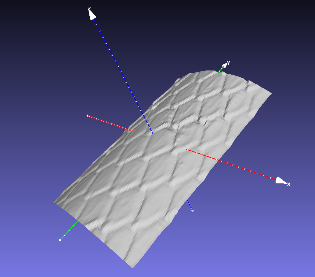
\includegraphics[scale=0.40]{derivation/structuregeom.png}
    \label{fig:strucgeom}
  }
~
  \subfigure[Nanostructure Surface]{
    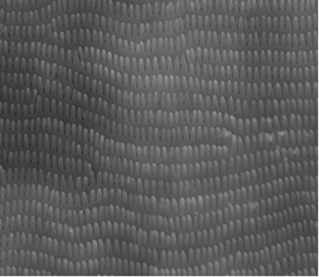
\includegraphics[scale=0.40]{derivation/nanostructuresurface.png}
    \label{fig:nanostruc}
  }
~
  \subfigure[Patch Orientation]{
    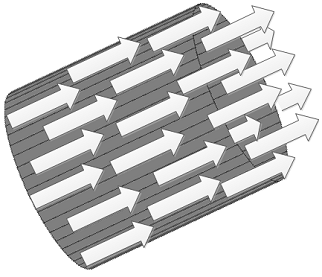
\includegraphics[scale=0.40]{derivation/vectorfieldalongcylinder.png}
    \label{fig:patchvectorfield}
  }
  \caption[Problem Statement]{Input for our simulation}
  \label{fig:problemstatement}
\end{figure}

We want to rely on the integral equation $\ref{eq:mainstam}$ derived by J. Stam in his paper $\cite{diffstam}$ about diffraction shaders. This equation formualtes a BRDF modeling the effect of diffraction under the assumption that a given grating can either be formulated as an analytical function or its structure is simple enough beeing modeled relying on statistical methods. These assumptions guarantee that $\ref{eq:mainstam}$ has an explicit solution. However, the complexisty of a biological nanostructures cannot sufficiently and accurately modeled simply using statistical methods. This is why interactive computation at high resolution becomes a hard task, since we cannot evaluate the given integral equation on the fly. Therefore, we have to adapt Stam's equation such that we are able to perform interactive rendering using explicitly provided height fields.

\begin{figure}[H]
  \centering
  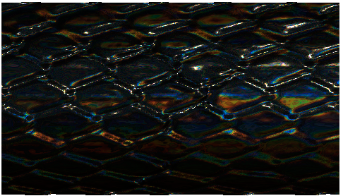
\includegraphics[scale=0.5]{derivation/renderedstructuredcolors.png}
  \caption[Problem Statement: Output]{Output: Rendered Structural Colors}
  \label{fig:problemstatementoutput}
\end{figure}


\section{Approximate a FT by a DFT}
\subsection{Reproduce FT by DTFT}
In the previous section, we have found an identity for the reflected spectral radiance $L_{\lambda}(\omega_r)$ when using Stam's BRDF for a given input height field. However, the derived expression in equation $\ref{eq:nonrelativebrdffinding}$ requires to evaluate the Fourier Transform of our height field$\footnote{actually it requires the computation of the inverse Fourier Transform of a transformed version of the given heightfield, the function p(x,y) defined in equation \ref{eq:px}.}$ for every direction. In this section we explain how to approximate the FT by the DTFT and apply it to our previous derivations. Figure $\ref{fig:ftbydtft}$ graphically shows how to obtain the DTFT from the FT for a one dimensional signal$\footnote{For our case we are dealing with a two dimensional, spatial signal, the given height field. Nevertheless, without any constraints of generality, the explained approach applies to multi dimensional problems.}$ \\ \\

\begin{figure}[ht]
  \centering
  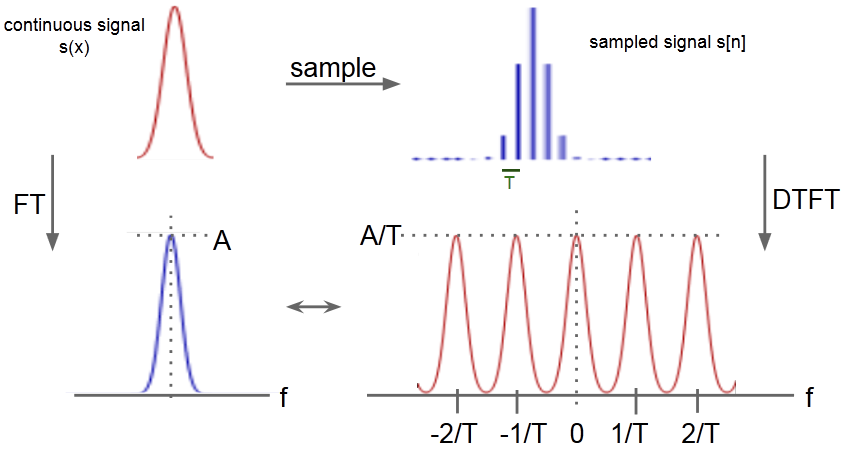
\includegraphics[scale=0.6]{derivation/ftbydtft.png}
  \caption[FT by DTFT]{Illustration of how to approximate the analytical Fourier Transform (FT) $\footnotemark$ of a given continuous signal by a Discrete Time Fourier Transform (DTFT).}
  \label{fig:ftbydtft}  
\end{figure}
\footnotetext{Images of function plots taken from \texttt{http://en.wikipedia.org/wiki/Discrete\textunderscore Fourier\textunderscore transform} and are modified.} 

The first step is to uniformly discretize the given signal since computers are working finite, discrete arithmetic. We rely on the Nyquist–Shannon sampling theorem tells us how dense we have to sample a given signal $s(x)$ such that can be reconstructed its sampled version $\hat{s}[n]$$\footnote{n denotes the number of samples.}$. In particular, a sampled version according to the Nyquist–Shannon sampling theorem will have the same Fourier Transform as its origianl singal. The sampling theorem states that if $f_{max}$ denotes the highest frequency of $s(x)$, then, it has to be sampled by a rate of $f_s$ with $2f_{max} \leq f_s$ in order to be reconstructable. By convention $T = \frac{1}{f_s}$ represent the interval length between two samples. \\ \\

Next, we apply the Fourier Tranformation operator on the discretized singal $\hat{s}$ which gives us the following expression: 

\begin{align}
\mathcal{F}_{FT}\{\hat{s}\}(w)
& = \int_{\mathds{R}} \hat{s}[n] e^{-iwx} dx \nonumber\\
& = \int_{\mathds{R}} mask(x)s(x) e^{-iwx} dx \nonumber\\
& = T\sum_{x=-\infty}^{\infty} \hat{s}[x] e^{-iwx} \nonumber\\
& = T\mathcal{F}_{DTFT}\{s\}(w)
\label{eq:sampledsignalfttodtft}
\end{align} 
Equation $\ref{eq:sampledsignalfttodtft}$ tells us that if $\hat{s}$ is sufficiently sampled, then its DTFT corresponds to the FT of $s(x)$ . Notice that the resulting DTFT from the sampled signal has a height of $\frac{A}{T}$ where A is the height of the FT of $s$ and thus is a scaled version of the FT.

\subsection{Spatial Coherence and Windowing}
Before we can derive a final expression in order to approximate a FT by a DFT, we first have to revisit the concept of coherence introduced in section $\ref{sec:wavecoherence}$ of chapter 2.Previousely we have seen that Stam's BRDf tells us what is the total contribution of all secondary sources which allows us to say what is the reflected spectral radiance at a certain point in space. This is related to stationary interference which itself depends on the coherence property of the emitted secondary wave sources. The ability for two points in space, $t_1$ and $t_2$, to interfere in the extend of a wave when being averages over time is the so called spatial coherence. The spatial distance between such two points over which there is significant intererence is limited by the quantity coherence area. For filtered sunlight on earth this is equal to 65$\mu m$ $\footnote{A proof for this number can be looked up in the book Optical Coherence and Quantum Optics$\cite{optcoherence}$ on page 153 and 154.}$.

\begin{figure}[H]
  \centering
  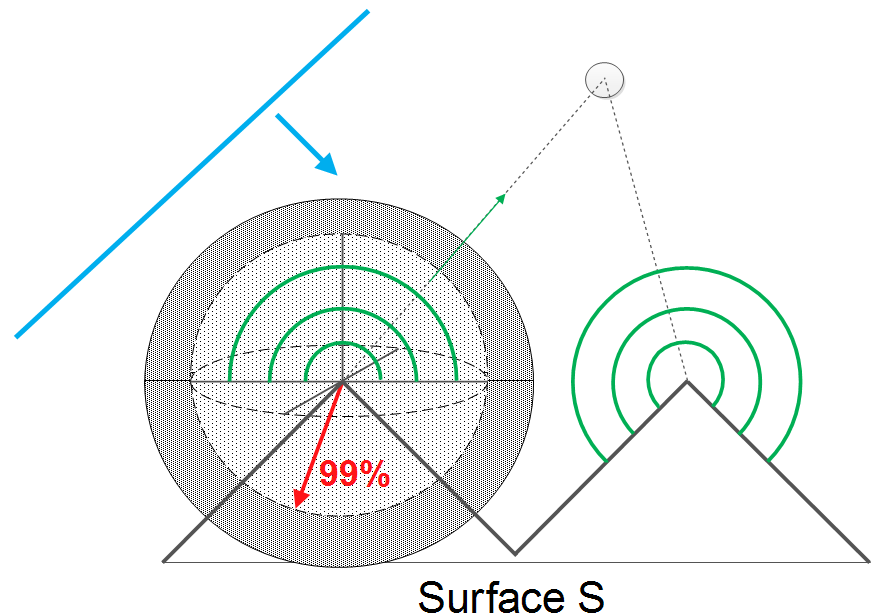
\includegraphics[scale=0.5]{derivation/windowinggaussian.png}
  \caption[Coherence Area using Gaussian Window]{A plane wave encoungers a surface. According to Huygens principle, secondary wavelets are emitted of from this surface. The resulting wave at a certain point in space (here indicated by a gray circle) depends on the inteference among all waves encountering at this position. The amount of significant interference is directly affected by the spatial coherence property of all the wavelets.}
  \label{fig:coherenceareagaussianwindow}  
\end{figure}

Figure $\ref{fig:coherenceareagaussianwindow}$ illustrates the concept of spatial coherence. A wavefront (blue line) encounters a surface. Due to Hugen's Principle, secondary wavelets are emitted off from the surface. The reflected radiance at a certain point in space, e.g. at a viewer's eye position (denoted by the gray circle), is a result of interference among all wavelets at that point. This interference is directly affected by the spatial coherence property of all the emitted wavelets. \\

In physics spatial coherence is predicted by the cross correlation between $t_1$ and $t_2$ and usually modeled by by a Gaussian Random Process. For any such Gaussian Processes we can use a spatial gaussian window $g(x)$ which is equal:

\begin{equation} 
  g(x) = \frac{1}{\sqrt{2\pi}\cdot\sigma}\cdot e^{-\frac{x^2}{2\sigma^2}} 
  \label{eq:gaussianwindowspacial}
\end{equation} 

We have chosen standard deviation $\sigma_s$ of the window such that it fulfills the equation $4 \sigma_s = 65\mu m$. This is equivalent like saying we want to predict about $99.99\%$$\footnote{Standard deviation values from confidence intervals table of normal distribution provided by Wolfram MatheWorld \texttt{http://mathworld.wolfram.com/StandardDeviation.html}.}$ of the resulting spatial coherence interference effects in our model by a cross correlation function. \\

By applying the Fourier Transformation to the spatial window we get the corresponding window in frequency space will look like:
\begin{equation} 
  \hat g(f) = e^{-\frac{f^2}{2\sigma_f^2}}
  \label{eq:gaussianwindowfrequencyspace}
\end{equation} 

Notice that this frequency space window has a standard deviation $\sigma_f$ equal to $\frac{1}{2 \pi \sigma_s}$. Those two windows, the spatial- and the frequency space window, will be used in the next section in order to approximate the DTFT by the DFT by a windowing apporach.

\subsection{Reproduce DTFT by DFT}
\label{sec:gaussianwindow}

MENTION CONVOLUTION THEOREM and explain its meaning and how it is used in this case
MENTION scales might not be appropriate

\begin{figure}[H]
  \centering
  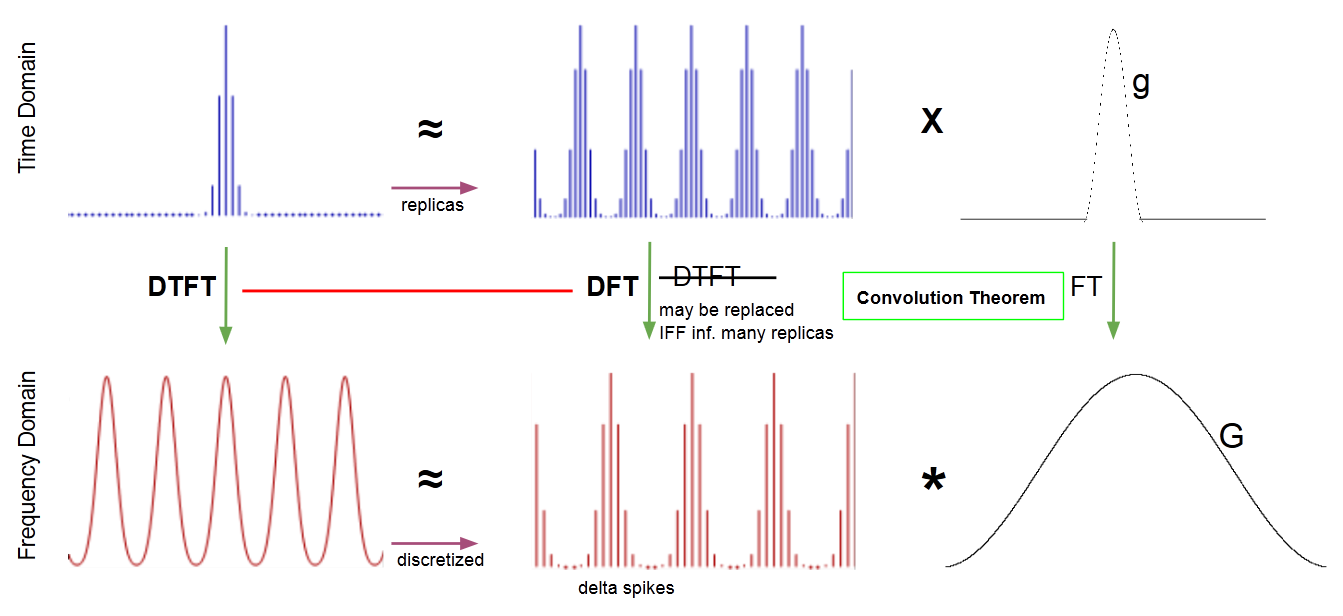
\includegraphics[scale=0.4]{derivation/dtftbydft.png}
  \caption[DTFT by DFT]{Illustration of how to approximate the DTFT $\footnotemark$ by the DFT.}
  \label{fig:dtftbydft}  
\end{figure}
\footnotetext{Images of function plots taken from \texttt{http://en.wikipedia.org/wiki/Discrete\textunderscore Fourier\textunderscore transform} and are modified.} 

Practically, we cannot compute the DTFT $\ref{eq:dtft}$ numerically due to finite computer arithmetic, since $w$ is a continuous function for the DTFT. The DFT $\ref{eq:dft}$ of a discrete height field patch is equivalent to the DTFT of an infinitely periodic function consisting of replicas of the same discrete patch. By windowing with a window function that is zero outside the central replica, the convolution of either the DFT or the DTFT of height field with the Fourier Transform of the window becomes equivalent.

Let $window_g$ denote the gaussian window with $4\sigma_s$ $\mu m$ where $\sigma_f = \frac{1}{2\pi\sigma_s}$
let us further substitute $\mathbf{t(x,y)}=i^n h(x,y)^n$

\begin{equation}
\mathcal{F}_{dtft}^{-1}\{\mathbf{t}\}(u,v) = \mathcal{F}_{fft}^{-1}\{\mathbf{t}\}(u,v)window_g(\sigma_f)
\end{equation} 

Therefore we can deduce the following expression from this:

\begin{align}
\mathcal{F}_{dtft}^{-1}\{\mathbf{t}\}(u,v)
& = \int_{-\infty}^{\infty} \int_{-\infty}^{\infty} {F}_{fft}^{-1}\{\mathbf{t}\}(w_u,w_v) \phi(u-w_u, v-w_v) dw_u dw_v \nonumber \\
& = \int_{-\infty}^{\infty} \int_{-\infty}^{\infty} \sum_i \sum_j {F}_{fft}^{-1}\{\mathbf{t}\}(w_u,w_v) \nonumber \\ 
& \quad \quad \delta(w_u-w_i, w_v-w_j)\phi(u-w_u, v-w_v) dw_u dw_v \nonumber \\
& = \sum_i \sum_j \int_{-\infty}^{\infty} \int_{-\infty}^{\infty}  {F}_{fft}^{-1}\{\mathbf{t}\}(w_u,w_v) \nonumber \\
& \quad \quad \delta(w_u-w_i, w_v-w_j)\phi(u-w_u, v-w_v) dw_u dw_v \nonumber \\
& = \sum_i \sum_j {F}_{fft}^{-1}\{\mathbf{t}\}(w_u,w_v) \phi(u-w_u, v-w_v)
\end{align}

where 

\begin{equation} \label{eq:gaussweight}
 \phi(x,y) = \pi e^{-\frac{x^2 + y^2}{2\sigma_{f}^2}}
\end{equation} 

%%%%%%%%%%%%%%%%%%%%%%%%%%%%%%%%%%%%%%%%%%%%%%%%%%%%%%%%%

\section{Adaption of Stam's BRDF discrete height fields}
\subsection{Rendering Equation}
As already discussed in the theoretical background chapter, colors are associated to radiance. Since we are starting with Stam's BRDF$\footnote{Remember that a BRDF is the portion of a incident light source reflected off a given surface towards a specified viewing direction}$ formulation but want to perform a simulation rendering structural colors, we have to reformulate this BRDF equation such that we will end up with an identity of the reflected spectral radiance. This is where the rendering equation comes into play. Lets assume we have given an incoming light source with solid angle $\omega_i$ and $\theta_i$ is its angle of incidence, $\omega_r$ is the solid angle for the reflected light. Further let $\lambda$ denote the wavelength and $\Omega$ is the hemisphere we of integration for the incoming light. Then, we are able to formulate a BRDF by using its definition $\ref{eq:defbrdf}$:  

\begin{alignat}{4}
& f_r(\omega_i, \omega_r) &&= \frac{dL_r(\omega_r)}{L_i(\omega_i)cos(\theta_i)d\omega_i} \nonumber \\
\Rightarrow{} & f_r(\omega_i, \omega_r) L_i(\omega_i)cos(\theta_i)d\omega_i &&= dL_r(\omega_r) \nonumber \\
\Rightarrow{} & \int_{\Omega}f_r(\omega_i, \omega_r) L_i(\omega_i)cos(\theta_i)d\omega_i &&= \int_{\Omega}dL_r(\omega_r) \nonumber\\
\Rightarrow{} & L_r(\omega_r) &&= \int_{\Omega}f_r(\omega_i, \omega_r) L_i(\omega_i)cos(\theta_i)d\omega_i
\label{eq:initialbrdf}
\end{alignat}

The last equation is the so called rendering equation $\label{sec:dirlighsourceassumption}$. We assume that our incident light is a directional, unpolarized light source $\ref{fig:dirlightsource}$ like sunlight and therefore its radiance is given as 

\begin{equation}
 L_{\lambda}(\omega)=I(\lambda)\delta(\omega-\omega_i)
\label{eq:radiancedirlightsource}
\end{equation}

where $I(\lambda)$ is the intensity of the relative spectral power for the wavelength $\lambda$. 
Since all light rays are parallel, whenever we are provided by a directional light source and we can think of radiance as a measure of the light emitted from a particular surface location into a particular direction, above's radiance identity will follow immediately. By plugging the identity $\ref{eq:radiancedirlightsource}$ into our current rendering equation $\ref{eq:initialbrdf}$, we will get:

\begin{align}
L_{\lambda}(w_r) 
& = \int_{\Omega} BRDF_{\lambda}(\omega_i, \omega_r) L_{\lambda}(\omega_i) cos(\theta_i) d\omega_i \nonumber \\
& = BRDF_{\lambda}(\omega_i, \omega_r) I(\lambda) cos(\theta_i)
\label{eq:deribrdfwithdirsource}
\end{align}

where $L_{\lambda}(\omega_i)$ is the incoming radiance and $L_{\lambda}(\omega_r)$ is the radiance reflected by the given surface. Note that the integral in equation $\ref{eq:deribrdfwithdirsource}$ vanishes since $\delta(\omega-\omega_i)$ is only equal one if and only if $\omega = \omega_i$.

\subsection{Reflected Radiance of Stam's BRDF}
We are going to use Stam's main derivation $~\eqref{eq:mainstam}$ for the $BRDF(\omega_i, \omega_r)$ in $\ref{eq:deribrdfwithdirsource}$ by applying the fact that the wavenumber is equal $k=\frac{2\pi}{\lambda}$:

\begin{align}
BRDF(\omega_i, \omega_r) 
& = \frac{k^2 F^2 G}{4\pi^2 A w^2} \langle \left|P(ku, kv) \right|^2\rangle \nonumber\\
& = \frac{4 \pi^2 F^2 G}{4\pi^2 A \lambda^2 w^2} \langle \left|P(ku, kv)  \right|^2\rangle \nonumber\\
& = \frac{F^2 G}{A \lambda^2 w^2} \langle \left|P(\frac{2\pi u}{\lambda}, \frac{2\pi v}{\lambda})  \right|^2\rangle
\label{eq:minoradaptedstam}
\end{align}

Going back to equation $\ref{eq:deribrdfwithdirsource}$ and plugging equation $\ref{eq:minoradaptedstam}$ into it, using the definition of equation $\ref{eq:geometricterm}$ and the equation $\ref{eq:sphericalomega}$ for $\omega$ we will get the following:

\begin{align}
L_{\lambda}(\omega_r) 
& = \frac{F^2 (1 + \omega_i \cdot \omega_r)^2}{A \lambda^2 cos(\theta_i)cos(\theta_r)  \omega^2} \left \langle \left|P \left( \frac{2\pi u}{\lambda}, \frac{2\pi v}{\lambda}\right) \right|^2 \right \rangle cos(\theta_i) I(\lambda) \nonumber \\
& = I(\lambda) \frac{F^2 (1 + \omega_i \cdot \omega_r)^2}{\lambda^2 A \omega^2 cos(\theta_r)} \left \langle \left|P \left( \frac{2\pi u}{\lambda}, \frac{2\pi v}{\lambda}\right) \right|^2 \right \rangle
\label{eq:nonrelativebrdffinding}
\end{align}

Note that the Fresnel term $F$ is actually a function of $(w_i, w_r)$, but in order to keep the equations simple, we omitted its arguemts. 
So far we just plugged Stam's BRDF identity into the rendering equation and hence have not significantly deviated from his formulation. Keep in mind that $P$ deontes the Fourier transform of the provided height field which depends on the viewing and incidence light direction. Thus this Fourier Transform has to be recomputed for every direction which will slow down the whole computation quite a lot$\footnote{Even a fast variant of computation the Fourier Transform has a runtime complexitiy of O(N log N) where N is the number of sample.}$. One particular strategy to solve this issue is to approximate $P$ by the Discrete Fourier Transform (DFT)$\footnote{See appendix \ref{chap:appendixsignalprocessing} for further information about different kinds of fourier transformations.}$ and seperate its computation such that terms for many directions can be precomputed and then later retrieved by look ups. The approximation of $P$ happens in two steps: First we approximate the Fourier Transform by the Discrete Time Fourier Transform (DTFT) and then, afterwards, we approximate the DTFT by the DFT. For further about basics of signal processing and Fourier Transformations please consult the appendix $\ref{chap:appendixsignalprocessing}$. \\

Using the insight gained by equation $\ref{eq:sampledsignalfttodtft}$ allows us to further simplify equation $\ref{eq:nonrelativebrdffinding}$:

\begin{align}
L_{\lambda}(\omega_r) 
& = I(\lambda) \frac{F^2 (1 + \omega_i \cdot \omega_r)^2}{\lambda^2 A w^2 cos(\theta_r)} \left \langle \left|P \left( \frac{2\pi u}{\lambda}, \frac{2\pi v}{\lambda}\right) \right|^2 \right \rangle \nonumber \\
& = I(\lambda) \frac{F^2 (1 + \omega_i \cdot \omega_r)^2}{\lambda^2 A w^2 cos(\theta_r)} \left \langle \left|T^2 P_{dtft}\left( \frac{2\pi u}{\lambda}, \frac{2\pi v}{\lambda}\right) \right|^2 \right \rangle
\label{eq:nonrelativebrdffindingreproddtft}
\end{align}

Where $P_{dtft}$ is a substitude for $\mathcal{F}_{DTFT}\{s\}(w)$. Furthermore $T$ the sampling distance for the discretization of $p(x,y)$ assuming equal and uniform sampling in both dimensions $x$ and $y$.

\subsection{Relative Reflectance}
In this section we are going to explain how to scale our BRDF formulation such that all of its possible output values are mapped into the range $\left[0,1\right]$. Such a relative reflectance formulation will ease our life for later rendering purposes since usually color values are within the range $\left[0,1\right]$, too. Furthermore, this will allow us to properly blend the resulting illumination caused by diffraction with a texture map.

Let us examine what $L_\lambda(\omega_r)$ will be for $\omega_r = \omega_0 := (0,0,*)$ i.e. specular reflection case, denoted as $L_\lambda^{spec}(\omega_0)$. When we know the expression for $L_\lambda^{spec}(\omega_0)$ we would be able to compute the relative reflected radiance for our problem $\ref{eq:nonrelativebrdffinding}$ by simply taking the fraction between $L_\lambda(\omega_r)$ and $L_\lambda^{spec}(\omega_0)$ which is denoted by: 

\begin{equation}
  \rho_\lambda(\omega_i,\omega_r) = \frac{L_\lambda(\omega_r)}{L_\lambda^{spec}(\omega_0)}
  \label{eq:rohrel}
\end{equation}


Going back to the definition $\ref{eq:uvw}$ of $(u,v,w)= -\omega_i - \omega_r$ and using spherical coordinates $\ref{eq:sphericalcoordinates}$, we get for $w$ the following identity

\begin{align}
w 
&= -\omega_i - \omega_r \nonumber \\ 
&= -(\omega_i + \omega_r) \nonumber \\
&= -\left( cos(\theta_i)+cos(\theta_r) \right) 
\label{eq:sphericalomega}
\end{align}

and therefore $w^2$ is equal $(cos(\theta_i)+cos(\theta_r))^2$. 

But first, let us derive the following expression:

\begin{align}
L_\lambda^{spec}(\omega_0) 
& = I(\lambda) \frac{F(\omega_0, \omega_0)^2 (1+\colvec[0]{0}{1}\cdot\colvec[0]{0}{1})^2}{\lambda^2 A (cos(0)+cos(0))^2 cos(0)} \langle \left|T_0^2 P_{dtft}(0,0)  \right|^2\rangle \nonumber \\
& = I(\lambda) \frac{F(\omega_0, \omega_0)^2 (1+1)^2}{\lambda^2 A (1+1)^2 1}\left| T_0^2 N_{sample} \right|^2 \nonumber \\
& = I(\lambda) \frac{F(\omega_0, \omega_0)^2}{\lambda^2 A}\left| T_0^2 N_{sample} \right|^2 
\label{eq:lspec}
\end{align}

Where $N_{samples}$ is the number of samples of the DTFT $\ref{eq:dtft}$. Thus, we can plug our last derived expression $\ref{eq:lspec}$ into the definition for the relative reflectance radiance $\ref{eq:rohrel}$ in the direction $w_r$ and will get:

\begin{align}
\rho_\lambda(\omega_i,\omega_r)
& = \frac{L_\lambda(\omega_r)}{L_\lambda^{spec}(\omega_0)} \nonumber \\
& = \frac{I(\lambda) \frac{F(\omega_i, \omega_r)^2 (1 + \omega_i \cdot \omega_r)^2}{\lambda^2 A (cos(\theta_i)+cos(\theta_r))^2 cos(\theta_r)} \langle \left|T_0^2 P_{dtft}(\frac{2\pi u}{\lambda}, \frac{2\pi v}{\lambda}) \right|^2\rangle}{I(\lambda) \frac{F(\omega_0, \omega_0)^2}{\lambda^2 A}\left| T_0^2 N_{sample} \right|^2 } \nonumber \\
& = \frac{F^2(\omega_i,\omega_r)(1 + \omega_i \cdot \omega_r)^2}{F^2(\omega_0,\omega_0)(cos(\theta_i)+cos(\theta_r))^2 cos(\theta_r)} \langle \left|\frac{P_{dtft}(\frac{2\pi u}{\lambda}, \frac{2\pi v}{\lambda})}{N_{samples}}\right|^2\rangle
\label{eq:lspecrohrel}
\end{align}

For simplification and a better overview, let us introduce the following expression, the so called gain-factor:

\begin{equation} 
    C(\omega_i,\omega_r) = \frac{F^2(\omega_i,\omega_r)(1 + \omega_i \cdot \omega_r)^2}{F^2(\omega_0,\omega_0)(cos(\theta_i)+cos(\theta_r))^2 cos(\theta_r) N_{samples}^2}
\label{eq:cfact}
\end{equation}

Using this substitute, we will end up with the following expression for the relative reflectance radiance from equation $\ref{eq:lspecrohrel}$:

\begin{equation}
\rho_\lambda(\omega_i,\omega_r) =  C(\omega_i,\omega_r) \langle \left|P_{dtft}(\frac{2\pi u}{\lambda}, \frac{2\pi v}{\lambda})\right|^2\rangle
\label{eq:cpterm}
\end{equation}

Using the previous definition for the relative reflectance radiance $\ref{eq:rohrel}$:

\begin{equation}
 \rho_\lambda(\omega_i,\omega_r) = \frac{L_\lambda(\omega_r)}{L_\lambda^{spec}(\omega_0)} 
\end{equation}

Which we can rearrange to the expression: 

\begin{equation}
L_\lambda(\omega_r) = \rho_\lambda(\omega_i,\omega_r)L_\lambda^{spec}(\omega_0)
\label{eq:radianceomegarspec}
\end{equation}

Let us choose $L_\lambda^{spec}(w_0) = S(\lambda)$ such that is has the same profile as the relative spectral power distribution of CIE Standard Illuminant $D65$ discussed in $\ref{subsec:colortransformations}$. Furthermore, when integrating over $\lambda$ for a specular surface, we should get $CIE_{XYZ}$ values corresponding to the white point for $D65$. The corresponding tristimulus values using CIE colormatching functions $\ref{eq:tristimulusvalues}$ for the $CIE_{XYZ}$ values look like:

\begin{align}
X = \int_{\lambda}L_\lambda(\omega_r)\overline{x}(\lambda)d\lambda \nonumber \\
Y = \int_{\lambda}L_\lambda(\omega_r)\overline{y}(\lambda)d\lambda \nonumber \\
Z = \int_{\lambda}L_\lambda(\omega_r)\overline{z}(\lambda)d\lambda
\label{eq:tristimrad}
\end{align}

where $\overline{x}$, $\overline{y}$, $\overline{z}$ are the color matching functions. Using our last finding $\ref{eq:radianceomegarspec}$ for $L_\lambda(\omega_r)$ with the definition for the tristimulus values $\ref{eq:tristimrad}$, we can actually derive an expression for computing the colors for our initial BRDF formula $\ref{eq:initialbrdf}$. 
Without any loss of generality it satisfies to derive an explicit expression for just one tristimulus term, for example X. Since The other have a similar formulation, except the we have to replace all X with Y or Z respectively. Therefore, we get:

\begin{align}
X 
& =\int_{\lambda}L_\lambda(\omega_r)\overline{x}(\lambda)d\lambda \nonumber \\
& =\int_{\lambda}\rho_\lambda(\omega_i,\omega_r)L_\lambda^{spec}(\omega_0) \overline{x}(\lambda)d\lambda \nonumber \\
& =\int_{\lambda}\rho_\lambda(\omega_i,\omega_r) S(\lambda) \overline{x}(\lambda)d\lambda \nonumber \\
& =\int_{\lambda} C(\omega_i,\omega_r) \langle \left|P_{dtft}(\frac{2\pi u}{\lambda}, \frac{2\pi v}{\lambda})\right|^2\rangle S(\lambda) \overline{x}(\lambda)d\lambda \nonumber \\
& = C(\omega_i,\omega_r) \int_{\lambda} \langle \left|P_{dtft}(\frac{2\pi u}{\lambda}, \frac{2\pi v}{\lambda})\right|^2\rangle S(\lambda) \overline{x}(\lambda)d\lambda \nonumber \\
& = C(\omega_i,\omega_r) \int_{\lambda} \langle \left|P_{dtft}(\frac{2\pi u}{\lambda}, \frac{2\pi v}{\lambda})\right|^2\rangle S_x(\lambda)d\lambda
\end{align}

Where we used the definition $S_x(\lambda)\overline{x}(\lambda)$ in the last step.

\section{Optimization using Taylor Series}
\label{sec:taylorapproximation}
In this section, we will deliver an approximation for the inverse Fourier Transformation of Stam's auxiliary function $p(x,y)$. This derivation will rely on the definition of Taylor Series expansion $\ref{eq:deftaylor}$. Further, we will provide an error bound for our approximation approach for a given number of iterations. Last, we will extend our current BRDF formula by the findings derived within this section.

Given $p(x,y)=e^{ikwh(x,y)}$ form Stam's Paper $\ref{sec:sumstam}$ where $h(x,y)$ is a given height field. Let be y real or even complex value, and lets consider the power series for the the exponential function
 
\begin{equation}
  e^{t}=1+t+\frac{t^{2}}{2!}+\frac{t^{3}}{3!}+...=\sum_{n=0}^{\infty}\frac{t^{n}}{n!}
\end{equation}

Let us define 
\begin{align}
t 
= t(x,y) 
= ikwh(x,y)
\end{align}
 
where $i$ is the imaginary number. For simplification, let us denote $h(x,y)$ as $h$. Then it follows by our previous stated identities: 

\begin{align}
 e^{t}
 &=1+(ikwh)+\frac{1}{2!}(ikwh)^{2}+\frac{1}{3!}(ikwh)^{3}+... \nonumber \\
 &=\sum_{n=0}^{\infty}\frac{(ikwh)^{n}}{n!}.
\end{align}

Hence it holds $p(x,y)=\sum_{n=0}^{\infty}\frac{(ikwh(x,y))^{n}}{n!}$. Let us now compute the Fourier Transformation of p(x,y) form above:

\begin{align}
  \mathcal{F}\left\{ p\right\}(u,v)
  & =\mathcal{F}\left\{ \sum_{n=0}^{\infty}\frac{(ikwh)^{n}}{n!}.\right\}(u,v) \nonumber \\
  & =^{\mathcal{F}\, lin\, Operator}\sum_{n=0}^{\infty}\mathcal{F}\left\{ \frac{(ikwh)^{n}}{n!}\right\}(u,v) \nonumber \\
  & =\sum_{n=0}^{\infty}\frac{(ikw)^{n}}{n!}\mathcal{F}\left\{ h{}^{n}\right\}(u,v)
\end{align}

Therefore it follows: $P(\alpha,\beta)=\sum_{n=0}^{\infty}\frac{(ikw)^{n}}{n!}\mathcal{F}\left\{ h{}^{n}\right\} (\alpha,\beta)$ for which $\mathcal{F}_{FT}\left\{ h{}^{n}\right\} (u,v)$.

Next we are going to look for an $N\mathbb{\in N}$ such that 
\begin{equation}
 \sum_{n=0}^{N}\frac{(ikwh)^{n}}{n!}\mathcal{F}\left\{ h{}^{n}\right\} (\alpha,\beta) \approx P(\alpha,\beta) 
\end{equation}

is a good approximation. But first the following two facts have to be proven:

\begin{enumerate}
\item Show that there exist such an $N\mathbb{\in N}$s.t the approximation
holds true.
\item Find a value for B s.t. this approximation is below a certain error
bound, for example machine precision $\epsilon$. 
\end{enumerate}

\myparagraph{Proof Sketch of 1.}

By the \textbf{ratio test} (see \textbf{{[}1{]}}) 
It is possible to show that the series $\sum_{n=0}^{N}\frac{(ikwh)^{n}}{n!}\mathcal{F}\left\{ h{}^{n}\right\} (\alpha,\beta)$ converges absolutely:

\textbf{Proof}: Consider $\sum_{k=0}^{\infty}\frac{y^{n}}{n!}$ where
$a_{k}=\frac{y^{k}}{k!}$. By applying the definition of the ratio test for this series it follows: 

\begin{equation}
 \forall y:limsup_{k\rightarrow\infty}|\frac{a_{k+1}}{a_{k}}|=limsup_{k\rightarrow\infty}\frac{y}{k+1}=0 
\end{equation}

Thus this series converges absolutely, no matter what value we will
pick for y.

\myparagraph{Part 2: Find such an N}
Let $f(x)=e^{x}$. We can formulate its Taylor-Series, stated above.
Let $P_{n}(x)$denote the n-th Taylor polynom, 

\begin{equation}
 P_{n}(x)=\sum_{k=0}^{n}\frac{f^{(k)}(a)}{k!}(x-a)^{k}
\end{equation}

where $a$ is our developing point (here a is equal zero). 

We can define the error of the n-th Taylor polynom to be $E_{n}(x)=f(x)-P_{n}(x)$.
the error of the n-th Taylor polynom is difference between the value of the function and the Taylor polynomial
This directly implies $|E_{n}(x)|=|f(x)-P_{n}(x)|$. By using the Lagrangian Error Bound it follows: 

\begin{equation}
 |E_{n}(x)|\leq\frac{M}{(n+1)!}|x-a|^{n+1} 
\end{equation}

with $a=0$, where \textbf{M} is some value satisfying $|f^{(n+1)}(x)|\leq M$ on the interval $I=[a,x]$. Since we are interested in an upper bound of the error and since \textbf{a} is known, we can reformulate the interval as $I=[0,x_{max}]$, where 

\begin{equation}
 x_{max} = \|i\| k_{max} w_{max} h_{max}
\end{equation}

We are interested in computing an error bound for $e^{ikwh(x,y)}$. Assuming the following parameters and facts used within Stam's Paper: 

\begin{itemize}
\item Height of bump: 0.15micro meters
\item Width of a bump: 0.5micro meters
\item Length of a bump: 1micro meters
\item $k=\frac{2\pi}{\lambda}$ is the wavenumber, $\lambda\in[\lambda_{min,}\lambda_{max}]$ and
thus $k_{max}=\frac{2\pi}{\lambda_{min}}$. Since $(u,v,w) = -\omega_i - \omega_r$ and both are unit direction vectors, 
each component can have a value in range {[}-2, 2{]}.
\item for simplification, assume$[\lambda_{min,}\lambda_{max}]=[400nm,700nm].$

\end{itemize}

We get:  

\begin{align}
x_{max}
 &= \|i\|*k_{max}*w_{max}*h_{max} \nonumber \\
 &= k_{max}*w_{max}*h_{max} \nonumber \\
 &=2*(\frac{2\pi}{4*10^{-7}m})*1.5*10^{-7} \nonumber \\
 &=1.5\pi
\end{align}

and it follows for our interval $I=[0,1.5\pi]$. 

Next we are going to find the value for $M$. Since the exponential function is monotonically growing (on the interval I) and the derivative of the \textbf{exp} function is the exponential function itself, we can find such an $M$: 
\begin{align*}
 M
 &=e^{x_{max}} \nonumber \\
 &=exp(1.5\pi)
\end{align*}

and $|f^{(n+1)}(x)|\leq M$ holds. With 

\begin{align}
|E_{n}(x_{max})|
 &\leq\frac{M}{(n+1)!}|x_{max}-a|^{n+1} \nonumber \\
 &= \frac{exp(1.5\pi)*(1.5\pi)^{n+1}}{(n+1)!}
\end{align}

we now can find a value of $n$ for a given bound, i.e. we can find an value of $N\mathbb{\in N}$ s.t. $\frac{exp(1.5\pi)*(1.5\pi)^{N+1}}{(N+1)!}\leq\epsilon$.
With Octave/Matlab we can see: 

\begin{itemize}
\item if N=20 then $\epsilon\approx2.9950*10^{-4}$
\item if N=25 then $\epsilon\approx8.8150*10^{-8}$
\item if N=30 then $\epsilon\approx1.0050*10^{-11}$
\end{itemize}

With this approach we have that $\sum_{n=0}^{25}\frac{(ikwh)^{n}}{n!}\mathcal{F}\left\{ h{}^{n}\right\} (\alpha,\beta)$ is
an approximation of $P(u,v)$ with error $\epsilon\approx8.8150*10^{-8}$. This means we can precompute 25 Fourier Transformations in order to approximate P(u,v) having an error $\epsilon\approx8.8150*10^{-8}$. 

Using now our approximation for $P_{dtft} = \mathcal{F}^{-1}\{p\}(u,v)$ for the tristimulus value X, we will get:

\begin{align}
X 
& = C(w_i,w_r) \int_{\lambda} \langle \left|P_{dtft}(\frac{2\pi u}{\lambda}, \frac{2\pi v}{\lambda})\right|^2\rangle S_x(\lambda)d\lambda \nonumber \\
& = C(w_i,w_r) \int_{\lambda} \left| \sum_{n=0}^N \frac{(wk)^n}{n!} \mathcal{F}^{-1}\{i^n h^n\}(\frac{2\pi u}{\lambda}, \frac{2\pi v}{\lambda})\right|^2 S_x(\lambda)d\lambda
\label{eq:xcolexpression}
\end{align}

\section{Spectral Rendering}
As the last step of our series of derivations, we plug all our findings together to one big equation in order to compute the color for each pixel on our mesh in the $CIE_{XYZ}$ colorspace. For any given heigh-field $h(x,y)$ representing a small patch of a nano structure of a surface and the direction vectors $w_s$ and $w_r$ from figure $\ref{fig:geometricsetup}$ the resulting color caused by the effect of diffraction can be computed like: Let 

\begin{equation}
P_{\lambda}(u,v) = {F}_{fft}^{-1}\{i^n h^n\}(\frac{2\pi u}{\lambda},\frac{2\pi v}{\lambda})
\end{equation}

Then our final expression using our previous derivations will look like:

\begin{equation}
\begin{split}
\colvec[X]{Y}{Z}& = C(\omega_i,\omega_r) \int_{\lambda} \sum_{n=0}^N  \frac{(wk)^n}{n!} \sum_{(r,s) \in \mathcal{N}_1(u,v)} \left| P_{\lambda}(u-w_r,v-w_s) \right|^2 \\
& \quad \quad  \phi(u-w_r, v-w_s) \colvec[S_x(\lambda)]{S_y(\lambda)}{S_z(\lambda)}d\lambda
\end{split}
\label{eq:finalexpression}
\end{equation}

where $\phi(x,y) = \pi e^{-\frac{x^2 + y^2}{2\sigma_{f}^2}}$ is the Gaussian window $\ref{sec:gaussianwindow}$.

\section{Alternative Approach}
\subsection{PQ factors}
\label{sec:pq}
In this section we are presenting an alternative approach to the previous Gaussian window approach 
$\ref{sec:gaussianwindow}$ 
in order to solve the issue working with $DTFT$ instead the $DFT$. We assume, that a given surface $S$ is covered by a number of replicas of a provided representative surface patch $f$. In a simplified, one dimensional scenario, mathematically speaking, $f$ is assumed to be a periodic function, i.e. $\forall x \in \mathds{R} : f(x) = f(x+nT)$, where $T$ is its period and $n \in \mathds{N}_{0}$. Thus, the surfaces can be written formally as:

\begin{equation}
  S(x) = \sum_{n=0}^N f(x+nT)
\label{eq:replicatedpatchsurface}
\end{equation}

What we are looking for is an identity for the inverse Fourier transform of our surface $S$, required in order to simplify the $(X,Y,Z)$ colors from $\ref{eq:xcolexpression}$:

\begin{align}
\mathcal{F}^{-1}\{S\}(w)
& =\int f(x) e^{iwx}dx \nonumber \\
& =\int_{-\infty}^{\infty} \sum_{n=0}^{N} f(x+nT) e^{iwx}dx \nonumber \\
& =\sum_{n=0}^{N} \int_{-\infty}^{\infty} f(x+nT) e^{iwx}dx
\label{eq:pqsinit}
\end{align}

Next, apply the following substitution $x+nT = y$ which will lead us to:

\begin{gather}
x=y-nT \nonumber \\
dx=dy
\label{eq:substitude1dpq}
\end{gather} 

Plugging this substitution back into equation $\ref{eq:pqsinit}$ we will get: 

\begin{align}
\mathcal{F}^{-1}\{S\}(w)
& =\sum_{n=0}^{N} \int_{-\infty}^{\infty} f(x+nT) e^{iwx}dx \nonumber \\
& =\sum_{n=0}^{N} \int_{-\infty}^{\infty} f(y) e^{iw(y-nT)}dy \nonumber \\
& =\sum_{n=0}^{N} e^{-iwnT} \int_{-\infty}^{\infty} f(y) e^{iwy}dy \nonumber \\
& =\sum_{n=0}^{N} e^{-iwnT} \mathcal{F}^{-1}\{f\}(w) \nonumber \\
& =\mathcal{F}^{-1}\{f\}(w) \sum_{n=0}^{N} e^{-iwnT}
\label{eq:pqsub}  
\end{align}

We used the fact that the exponential term $e^{-iwnT}$ is a constant factor when integrating along $dy$ and the identity for the inverse Fourier transform of the function $f$. Next, let us examine the series $\sum_{n=0}^N e^{-iwnT}$ closer:

\begin{align}
\sum_{n=0}^N e^{-uwnT}
& =\sum_{n=0}^N (e^{-uwT})^n \nonumber \\
& =\frac{1-e^{iwT(N+1)}}{1-e^{-iwT}}
\label{eq:pqgeometricseries}
\end{align}

We recognize the geometric series identity for the left-hand-side of equation $\ref{eq:pqgeometricseries}$. Since our series is bounded, we can simplify the right-hand-side of equation $\ref{eq:pqgeometricseries}$.

Note that $e^{-ix}$ is a complex number. Every complex number can be written in its polar form, i.e. 

\begin{equation}
e^{-ix} = cos(x) + i sin(x) 
\label{eq:polarform}
\end{equation}

Using the following trigonometric identities
\begin{gather}
cos(-x) = cos(x) \nonumber \\
sin(-x) = -sin(x)
\end{gather}

combined with $\ref{eq:polarform}$ we can simplify the series $\ref{eq:pqgeometricseries}$ even further to:

\begin{align}
\frac{1-e^{iwT(N+1)}}{1-e^{-iwT}}
& =\frac{1-cos(wT(N+1)) + i sin(wT(N+1)) }{1-cos(wT) + i sin(wT)}
\label{eq:pq1minusexp}
\end{align}

Equation $\ref{eq:pq1minusexp}$ is still a complex number, denoted as $(p+iq)$. Generally, every complex number can be written as a fraction of two complex numbers. This implies that the complex number $(p+iq)$ can be written as $(p+iq) = \frac{(a+ib)}{(c+id)}$ for any $(a+ib), (c+id) \neq 0$. Let us use the following substitutions: 

\begin{align}
a& := 1 - cos(wT(N+1))&
b& =sin(wT(N+1)) \nonumber \\
c& =1-cos(wT)&
d& =sin(wT)
\label{eq:pqabcdsubstitudes}
\end{align}

Hence, using $\ref{eq:pqabcdsubstitudes}$, it follows 

\begin{equation}
  \frac{1-e^{iwT(N+1)}}{1-e^{-iwT}} = \frac{(a+ib)}{(c+id)}
\end{equation}

By rearranging the terms, it follows $(a+ib) = (c+id)(p+iq)$ and by multiplying its right hand-side out we get the following system of equations:

\begin{align}
(cp-dq)& =a \nonumber \\
(dp + cq)& =b
\label{eq:cdadcn}
\end{align}

After multiplying the first equation of $\ref{eq:cdadcn}$ by $c$ and the second by $d$ and then adding them together, we get using the law of distributivity new identities for $p$ and $q$:

\begin{align}
p& =\frac{(ac+bd)}{c^2 + d^2} \nonumber \\
q& =\frac{(bc+ad)}{c^2 + d^2}
\label{eq:pq1}
\end{align}

Using some trigonometric identities and putting our substitution from $\ref{eq:pqabcdsubstitudes}$ for $a$, $b$, $c$, $d$ back into the current representation $\ref{eq:pq1}$ of $p$ and $q$ we will get:

\begin{align}
p& =\frac{1}{2}+\frac{1}{2}\left(\frac{cos(wTN)-cos(wT(N+1))}{1-cos(wT)}\right) \nonumber \\
q& =\frac{sin(wT(N+1))-sin(wTN)-sin(wT)}{2(1-cos(wT))}
\end{align}

Since we have seen, that $\sum_{n=0}^N e^{-uwnT}$ is a complex number and can be written as $(p+iq)$, we now know an explicit expression for $p$ and $q$. Therefore, the one dimensional inverse Fourier transform of $S$ is equal:

\begin{align}
\mathcal{F}^{-1}\{S\}(w)
& =\mathcal{F}^{-1}\{f\}(w) \sum_{n=0}^{N} e^{-iwnT} \nonumber \\
& = (p+iq) \mathcal{F}^{-1}\{f\}(w)  
\label{eq:mainfinding1d}
\end{align}


Now lets consider our actual problem description. Given a patch of a nanoscaled sureface snake shed represented as a two dimensional heightfield $h(x,y)$. We once again assume that this provided patch is representing the whole surface $S$ of our geometry by some number of replicas of itself. Therefore, $S(x,y) = \sum_{n=0}^{N} h(x+nT_1, y+mT_2)$, assuming the given height field has the dimensions $T_1$ by $T_2$. In order to derive an identity for the two dimensional inverse Fourier transformation of $S$ we can similarly proceed like we did to derive equation $\ref{eq:mainfinding1d}$.

\begin{align}
\mathcal{F}^{-1}\{S\}(w_1, w_2)
& = \int_{-\infty}^{\infty}\int_{-\infty}^{\infty} \sum_{n_2=0}^{N_1} \sum_{n_2=0}^{N_2} h(x_1 + n_1 T_1, x_2 + n_2 T_2) e^{iw(x_1 + x_2)}dx_1 dx_2 \nonumber \\
& = \int_{-\infty}^{\infty}\int_{-\infty}^{\infty} \sum_{n_2=0}^{N_1} \sum_{n_2=0}^{N_2} h(y_1, y_2) e^{iw((y_1 - n_1 T_1) + (y_2 + n_2 T_2))}dx_1 dx_2 \nonumber \\
& =\sum_{n_2=0}^{N_1} \sum_{n_2=0}^{N_2} \int_{-\infty}^{\infty}\int_{-\infty}^{\infty} h(y_1, y_2) e^{iw(y_1 + y_2)} e^{-iw(n_1 T_1 + n_2 T_2)}dy_1 dy_2 \nonumber \\
& =\sum_{n_2=0}^{N_1} \sum_{n_2=0}^{N_2} e^{-iw(n_1 T_1 + n_2 T_2)} \int_{-\infty}^{\infty}\int_{-\infty}^{\infty} Box(y_1, y_2) e^{iw(y_1 + y_2)} dy_1 dy_2 \nonumber \\
& =\left(\sum_{n_2=0}^{N_1} \sum_{n_2=0}^{N_2} e^{-iw(n_1 T_1 + n_2 T_2)}\right) \mathcal{F}^{-1}\{h\}(w_1,w_2) \nonumber \\
& =\left(\sum_{n_2=0}^{N_1} e^{-iw n_1 T_1}\right) \left(\sum_{n_2=0}^{N_2} e^{-iw n_2 T_2}\right) \mathcal{F}^{-1}\{h\}(w_1,w_2) \nonumber \\
& =(p_1 + i q_1)(p_2 + i q_2) \mathcal{F}^{-1}\{h\}(w_1,w_2) \nonumber \\
& =((p_1 p_2 - q_1 q_2) + i(p_1 p_2 + q_1 q_2)) \mathcal{F}^{-1}\{h\}(w_1,w_2) \nonumber \\
& =(p + iq) \mathcal{F}_{DTFT}^{-1}\{h\}(w_1,w_2)
\label{eq:pqmainfinding}
\end{align}

Where we have defined 

\begin{align}
p := (p_1 p_2 - q_1 q_2) \nonumber \\ 
q := (p_1 p_2 + q_1 q_2)
\label{eq:pqsubst2d}
\end{align}

For the identity of equation $\ref{eq:pqmainfinding}$ we made use of Green's integration rule which allowed us to split the double integral to the product of two single integrations. Also, we used the definition of the 2-dimensional inverse Fourier transform of the height field function. We applied a similar substitution like we did in $\ref{eq:substitude1dpq}$, but this time twice, once for $x_1$ and once for $x_2$ separately. The last step in equation $\ref{eq:pqmainfinding}$, substituting with $p$ and $q$ in equation $\ref{eq:pqsubst2d}$ will be useful later in the implementation. The insight should be, that the product of two complex numbers is again a complex number. We will have to compute the absolute value of $\mathcal{F}^{-1}\{S\}(w_1,w_2)$ which will then be equal $(p^2 + q^2)^{\frac{1}{2}}\left|\mathcal{F}^{-1}\{h\}(w_1,w_2)\right|$


\subsection{Interpolation}
\label{sec:sincinterpolation}

In $\ref{sec:pq}$ we have derived an alternative approach when we are working with a periodic signal instead using the gaussian window approach from $\sec{sec:gaussianwindow}$. Its main finding $\ref{eq:pqmainfinding}$ that we can just integrate over one of its period instead iterating over the whole domain. Nevertheless, this main finding is using the inverse DTFT. Since we are using 

We are interested in recovering an original analog signal $x(t)$ from its samples $x[t] = $ 

Therfore, for a given sequence of real numbers $x[n]$, representing a digital signal, its correspond continuous function is: 

\begin{equation}
  x(t) = \sum_{n=-\infty}^{\infty} x[n] sinc\left(\frac{t-nT}{T}\right)
\end{equation}

which has the Fourier transformation $X(f)$ whose non-zero values are confined to the region $|f| \leq \frac{1}{2T} = B$.
When $x[n]$ represents time samples at interval $T$ of a continuous function, then the quantity $f_s = \frac{1}{T}$ is known as its sample rate and $\frac{f_s}{2}$ denotes the Nyquist frequency. The sampling Theorem states that when a function has a Bandlimit B less than the Nyquist frequency, then $x(t)$ is a perfect reconstruction of the original function. 

\begin{figure}[ht]
  \centering
  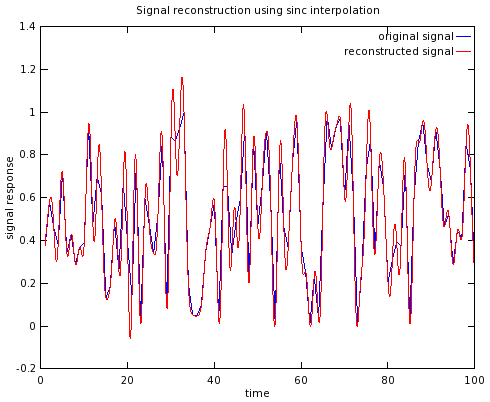
\includegraphics[scale=0.8]{background/sincreconstructed.png}
  \caption{Comparission between a given random one dimensional input signal $s(t)$ and its sinc interpolation $\hat{s}(t)$. Notice that for the interpolation there were $N=100$ samples from the original signal provided.}
  \label{fig:plotsincinterpolation}  
\end{figure}
